% !TeX root = these.tex
\newpage
\chapter*{Annexes}

\setcounter{page}{1}
\pagenumbering{roman}
%\pagenumbering{Roman}
%\pagenumbering{Arabic}




\section{Page de connexion et d'inscription}
\label{annexe/espace_nom}

\begin{figure}[!h]
	\begin{center}
		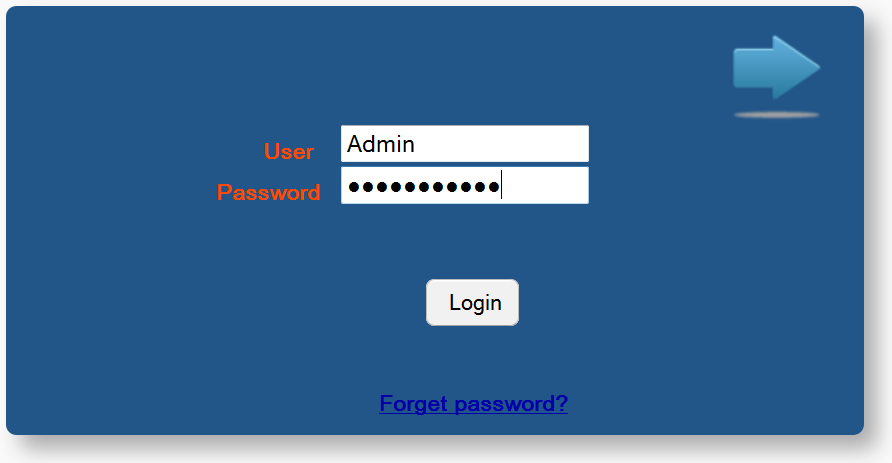
\includegraphics[width=12cm,height=6cm]{login.png}	
		\caption{page de connexion}
	\end{center}
\end{figure}

\begin{figure}[!h]
	\begin{center}
		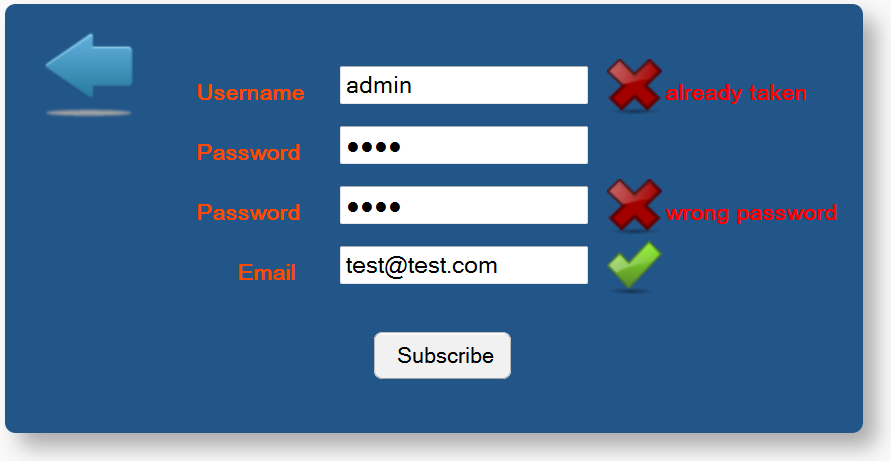
\includegraphics[width=12cm,height=6cm]{subscribe.png}
		\caption{page d'inscription}
	\end{center}
\end{figure}

\newpage

\section{Page des projets}
\label{annexe/espace_nom}

\begin{figure}[!h]
	\begin{center}
		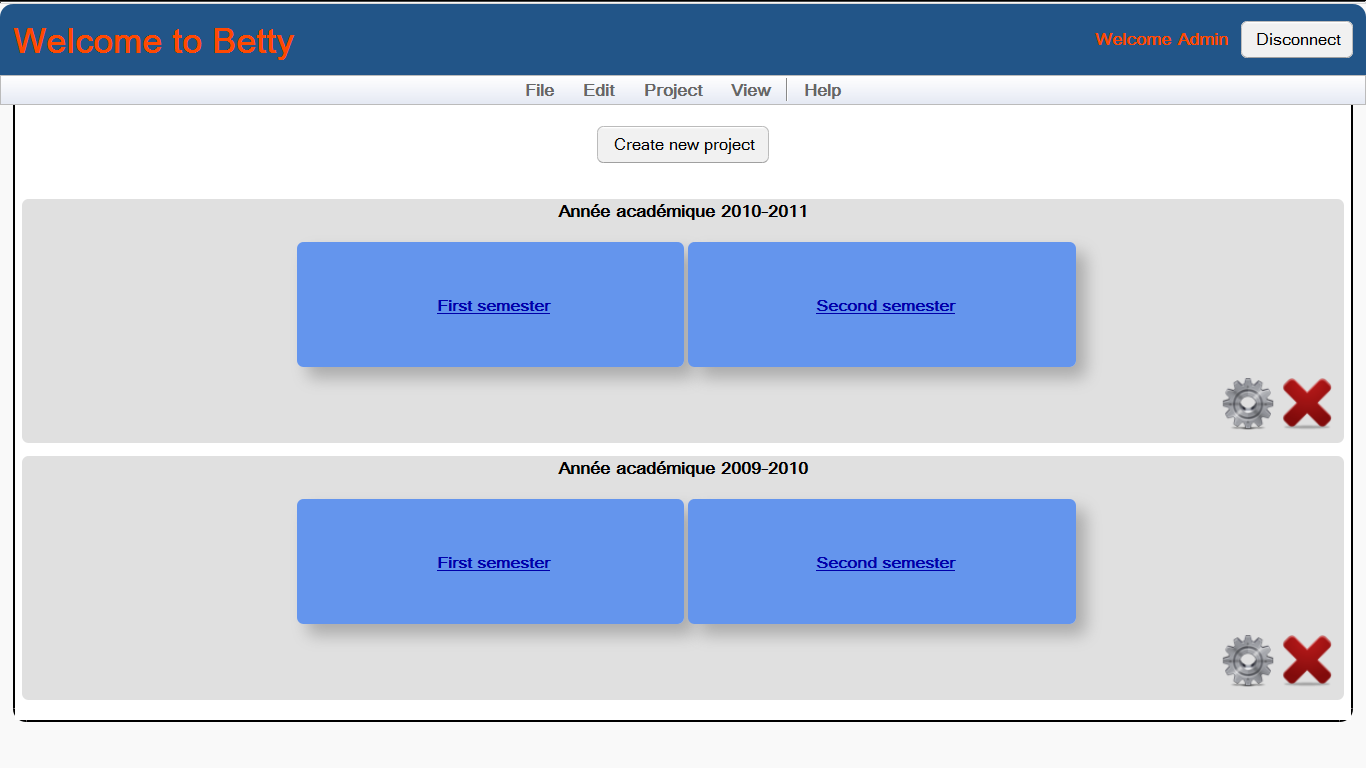
\includegraphics[width=19cm,height=12cm,angle=90]{ProjectPage.png}
		\caption{page des projets}
	\end{center}
\end{figure}\newpage

\newpage

\section{Page principale I}
\label{annexe/espace_nom}

\begin{figure}[!h]
	\begin{center}
		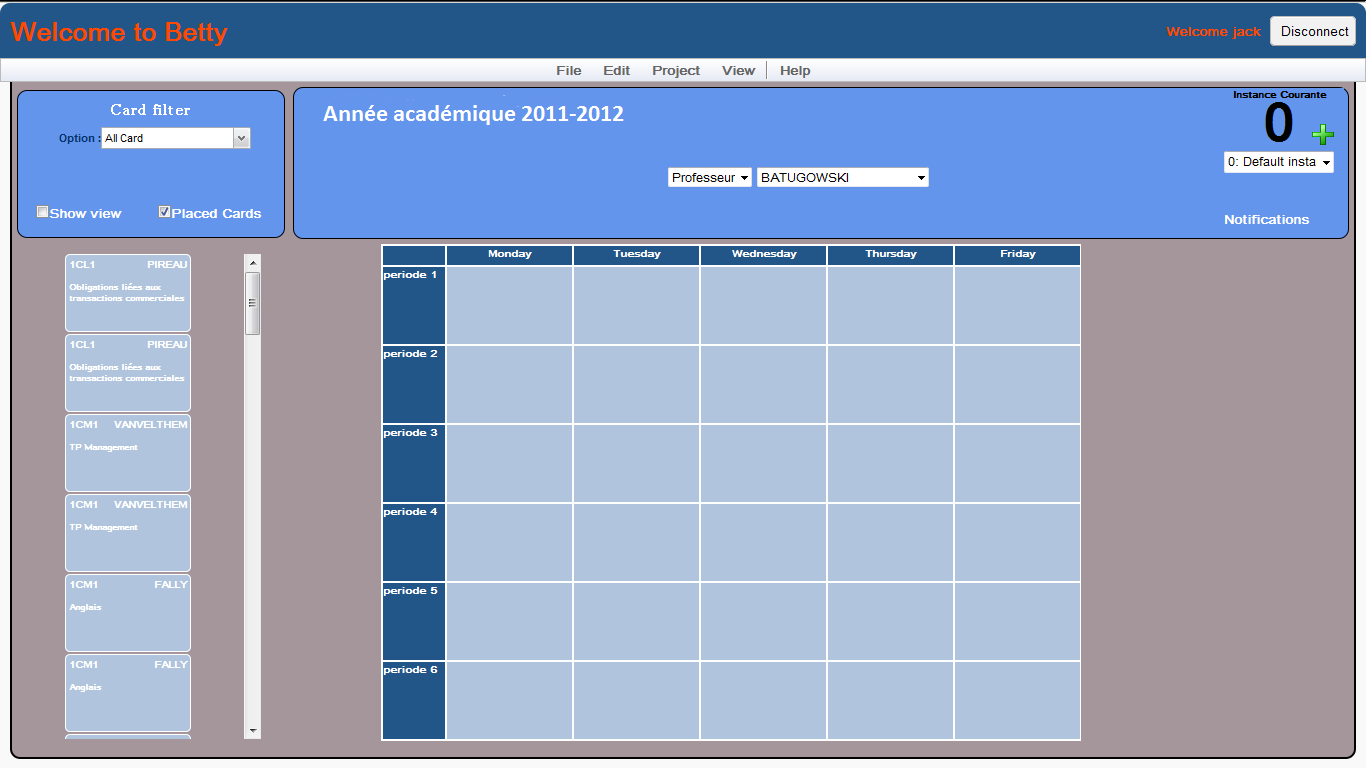
\includegraphics[width=19cm,height=12cm,angle=90]{MainPageClean.png}
		\caption{page principale vide}
	\end{center}
\end{figure}

\newpage

\section{Page principale II}
\label{annexe/espace_nom}

\begin{figure}[!h]
	\begin{center}
		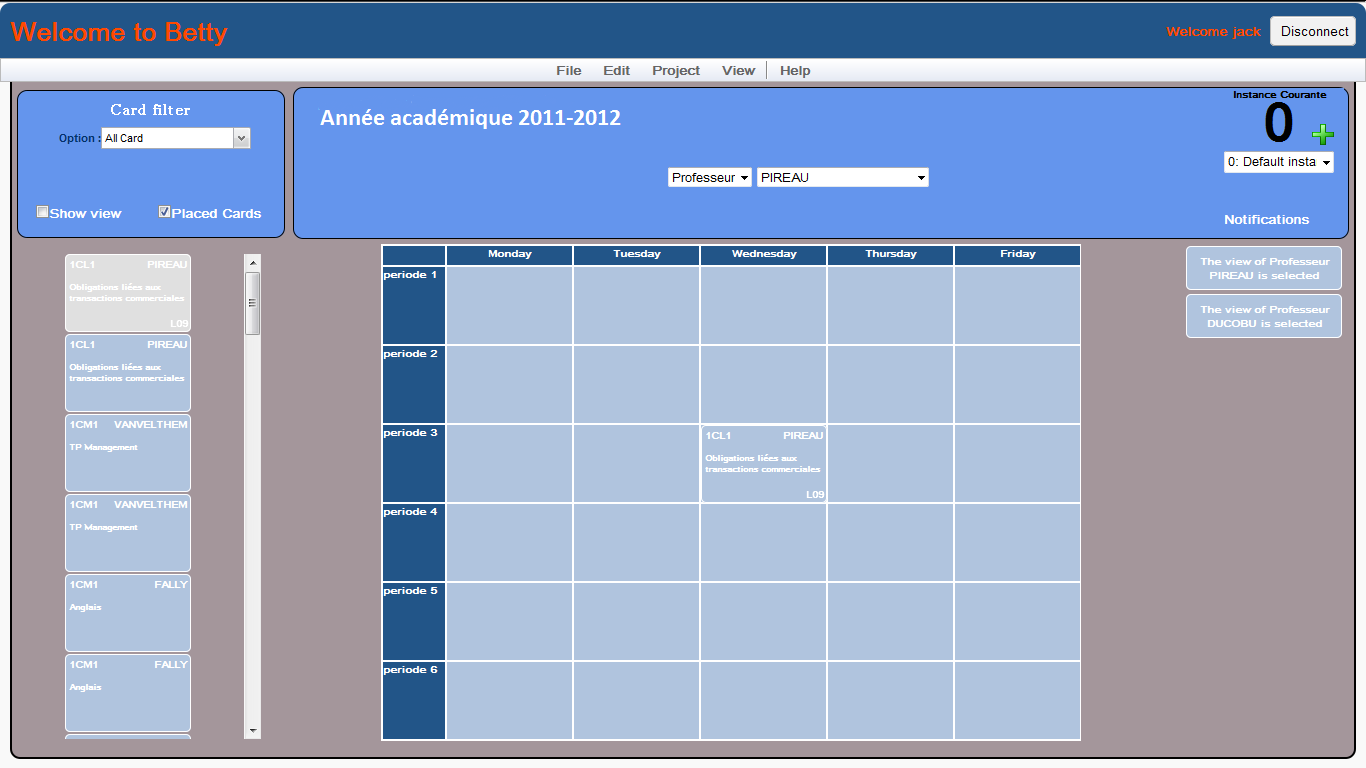
\includegraphics[width=19cm,height=12cm,angle=90]{MainPagePlacedCard.png}
		\caption{page principale carton placé}
	\end{center}
\end{figure}

\newpage

\section{Page principale III}
\label{annexe/espace_nom}

\begin{figure}[!h]
	\begin{center}
		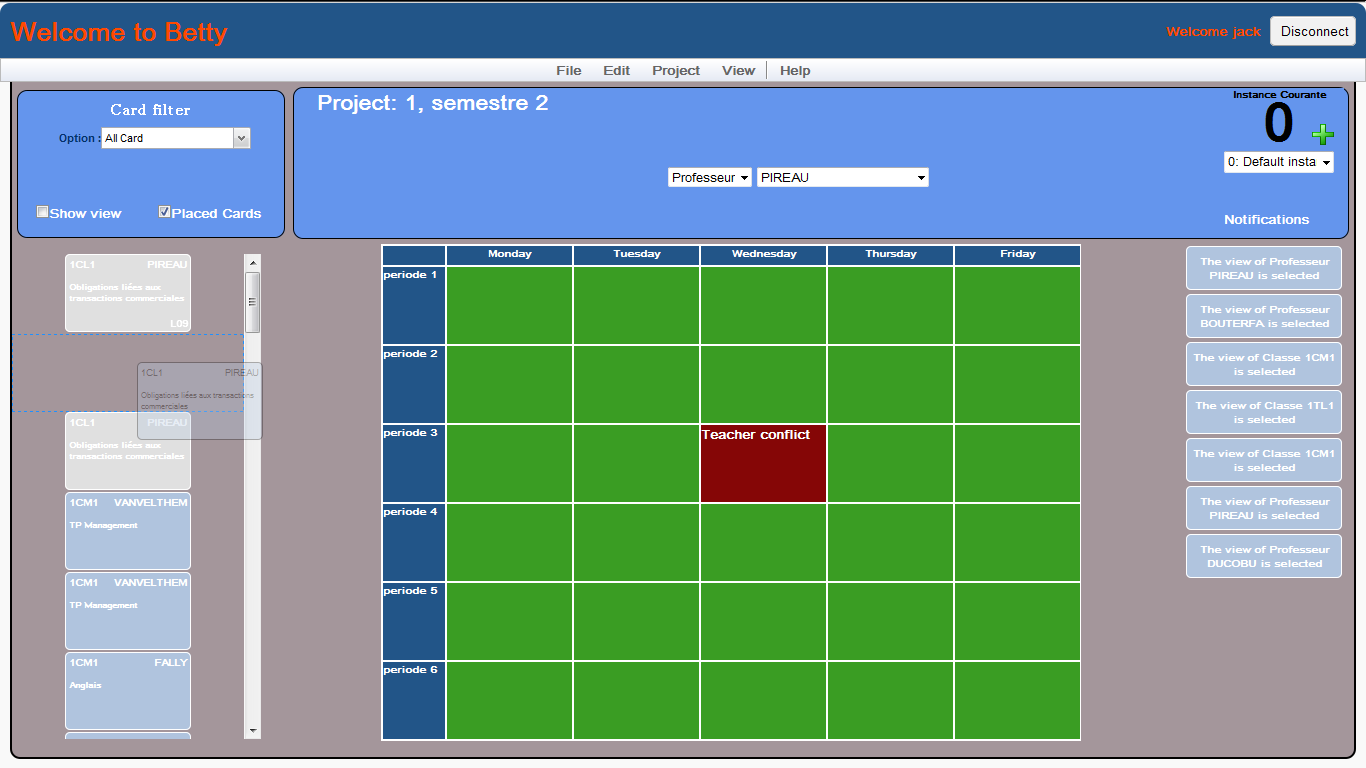
\includegraphics[width=19cm,height=12cm,angle=90]{MainPageColorTab.png}
		\caption{page principale solveur client}
	\end{center}
\end{figure}

\newpage

\section{Card filter}
\label{annexe/espace_nom}

\begin{figure}[!h]
	\begin{center}
		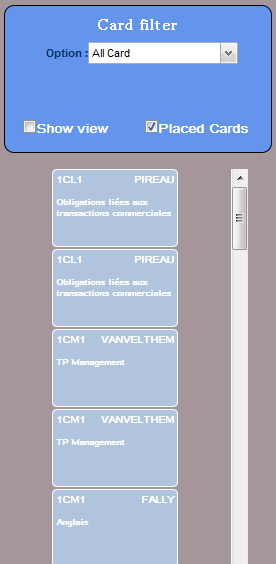
\includegraphics[width=6cm,height=12cm]{CardFilterAllCard.png}
		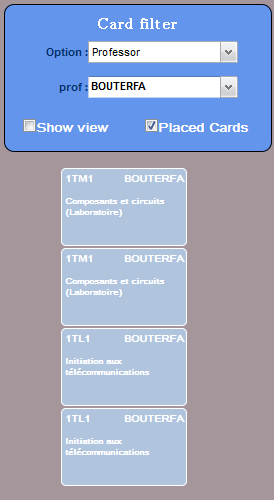
\includegraphics[width=6cm,height=10cm]{CardFilterBouterfa.png}
		\caption{présentation des cartons (non) filtrés}		
		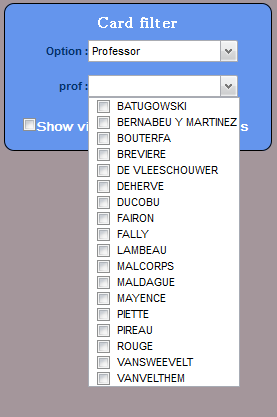
\includegraphics[width=6cm,height=8cm]{CardFIlterChoice.png}
		\caption{filtre avec multi-sélection}
	\end{center}
\end{figure}

\newpage

\section{Schéma entité association}
\label{annexe/espace_nom}

\begin{figure}[!h]
	\begin{center}
		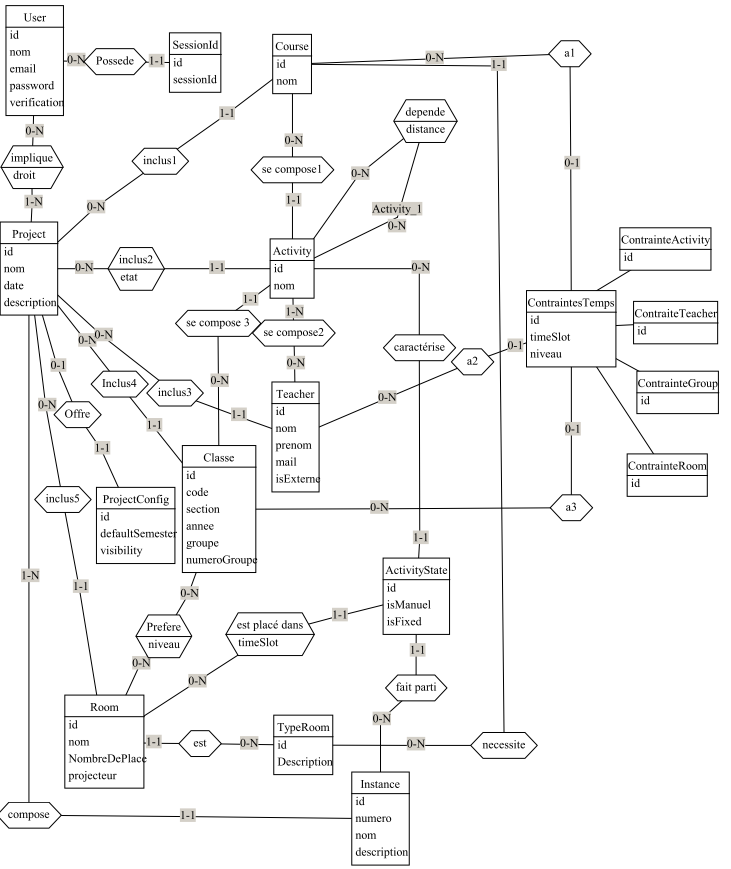
\includegraphics[width=15cm,height=19cm]{EA.png}
		\caption{concept de schéma de la base de données}
	\end{center}
\end{figure}
Celui-ci étant un concept, car nous avons travaillé avec des classes via le framework Hibernate.
